\documentclass[border=10pt]{standalone}
\usepackage[svgnames]{xcolor}
\usepackage{amsmath}
\usepackage{pgfplots}
\pgfplotsset{compat=newest}
\usepackage[sfdefault]{FiraSans}
\usepackage{FiraMono}
\renewcommand*\familydefault{\sfdefault}
\begin{document}
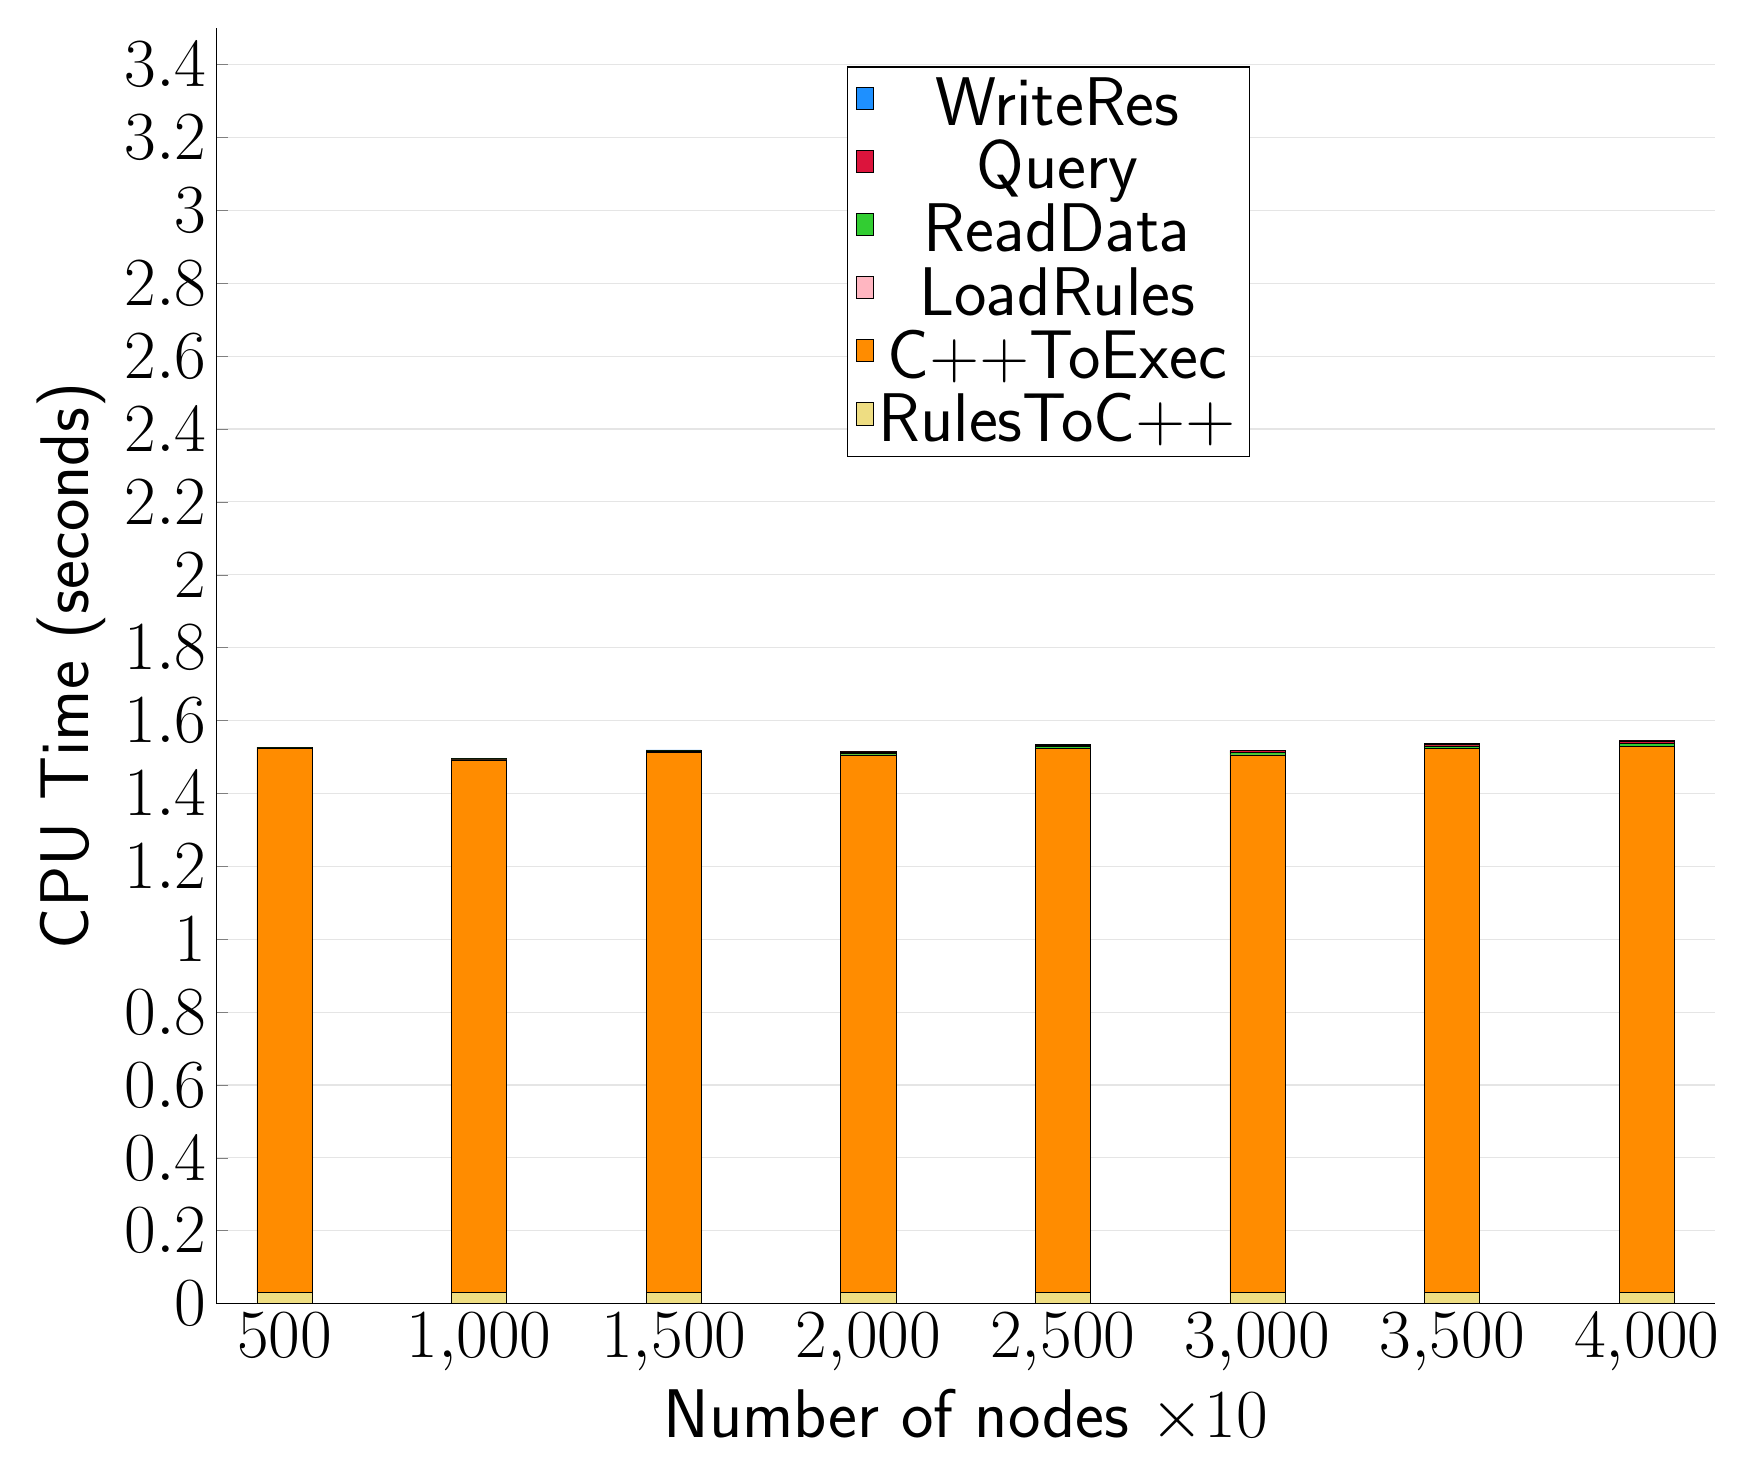
\begin{tikzpicture}
	\begin{axis}[
			ybar stacked,
			width=1.7\textwidth,
			bar width=0.7cm,
			ymajorgrids, tick align=inside,
			major grid style={draw=gray!20},
			xtick=data,
			ymin=0, ymax=3.5,
			axis x line*=bottom,
			axis y line*=left,
			enlarge x limits=0.05,
			legend style={
					at={(0.69, 0.97)},
					anchor=north east,
					legend columns=1,
					font=\Huge,
				},
			ylabel={CPU Time (seconds)},
			xlabel={Number of nodes $\times 10$},
			label style={font=\Huge},
			tick label style={font=\Huge},
		]
		\addlegendimage{fill=DodgerBlue, draw=black, line width=0.2pt}
		\addlegendentry{WriteRes}
		\addlegendimage{fill=Crimson, draw=black, line width=0.2pt}
		\addlegendentry{Query}
		\addlegendimage{fill=LimeGreen, draw=black, line width=0.2pt}
		\addlegendentry{ReadData}
		\addlegendimage{fill=LightPink, draw=black, line width=0.2pt}
		\addlegendentry{LoadRules}
		\addlegendimage{fill=DarkOrange, draw=black, line width=0.2pt}
		\addlegendentry{C++ToExec}
		\addlegendimage{fill=LightGoldenrod, draw=black, line width=0.2pt}
		\addlegendentry{RulesToC++}
		\addplot +[fill=LightGoldenrod, draw=black, line width=0.2pt] coordinates {
				(500, 0.031000000000000007)
				(1000, 0.030000000000000006)
				(1500, 0.030000000000000006)
				(2000, 0.030000000000000006)
				(2500, 0.030000000000000006)
				(3000, 0.030999999999999993)
				(3500, 0.030000000000000006)
				(4000, 0.030000000000000006)
			};
		\addplot +[fill=DarkOrange, draw=black, line width=0.2pt] coordinates {
				(500, 1.493)
				(1000, 1.4620000000000002)
				(1500, 1.483)
				(2000, 1.4760000000000002)
				(2500, 1.4940000000000002)
				(3000, 1.475)
				(3500, 1.493)
				(4000, 1.5)
			};
		\addplot +[fill=LightPink, draw=black, line width=0.2pt] coordinates {
				(500, 8.49e-05)
				(1000, 0.00011410000000000001)
				(1500, 0.0001239)
				(2000, 0.00010990000000000002)
				(2500, 8.26e-05)
				(3000, 9.669999999999999e-05)
				(3500, 8.04e-05)
				(4000, 0.00010779999999999999)
			};
		\addplot +[fill=LimeGreen, draw=black, line width=0.2pt] coordinates {
				(500, 0.0011630000000000002)
				(1000, 0.0025005)
				(1500, 0.0035295999999999995)
				(2000, 0.004693)
				(2500, 0.005098699999999999)
				(3000, 0.0065536)
				(3500, 0.0072546)
				(4000, 0.0081888)
			};
		\addplot +[fill=Crimson, draw=black, line width=0.2pt] coordinates {
				(500, 0.0006575000000000001)
				(1000, 0.0015742000000000002)
				(1500, 0.0022596999999999995)
				(2000, 0.003015)
				(2500, 0.0035719000000000007)
				(3000, 0.0044706)
				(3500, 0.0050712000000000005)
				(4000, 0.0056858)
			};
		\addplot +[fill=DodgerBlue, draw=black, line width=0.2pt] coordinates {
				(500, 0.00039709999999999995)
				(1000, 0.0006895)
				(1500, 0.0008583999999999999)
				(2000, 0.0010749000000000002)
				(2500, 0.001148)
				(3000, 0.0014338999999999999)
				(3500, 0.0015057999999999998)
				(4000, 0.0017131)
			};
	\end{axis}
\end{tikzpicture}

\end{document}
